\documentclass[conference]{IEEEtran}

\usepackage{amsmath,amssymb}
\usepackage{graphicx}
\usepackage{booktabs}
\usepackage[hidelinks]{hyperref}
\usepackage{subcaption}
\usepackage{siunitx}
\usepackage[ruled,vlined]{algorithm2e}
\usepackage{array}
\usepackage{multirow}
\usepackage{xcolor}
\usepackage{url}

% Convenience macros
\newcommand{\bm}[1]{\boldsymbol{#1}}
\newcommand{\norm}[1]{\left\lVert#1\right\rVert}
\newcommand{\dfree}{d_{\mathrm{free}}}

\title{Search Designed Trellis with Neural Decoding for Non-traditional Channels}

\author{\IEEEauthorblockN{Abhishek Manjunath}
\IEEEauthorblockA{Department of Electrical Engineering\\
University of Southern California\\
\texttt{akmanjun@usc.edu}}}

\begin{document}

\maketitle

% ============================================================
\begin{abstract}
Industrial-IoT and unlicensed sub-GHz wireless links share spectrum with
narrowband emissions from variable-frequency motor drives, switching power
converters, and PWM controllers, which appear at the receiver as periodic
sinusoidal interferers superimposed on thermal noise.  Under such
non-Gaussian interference, the standard mismatched soft-decision Viterbi
decoder for a rate-$1/2$, constraint-length-7 (NASA K=7) convolutional code
saturates at block-error rate (BLER) $=1$ for moderate interference levels.
I study learned and search-based co-design of the trellis and decoder
under a strict $2.1$~MFLOP/block compute budget representative of edge
radios.  A neural branch-metric estimator (\textbf{N2}, $\approx 1.86$\,k
parameters) trained against the oracle log-likelihood, plugged into a
standard Viterbi add-compare-select, achieves
BLER\,$=2.5{\times}10^{-3}$ at SNR\,$=$\,INR\,$=5$~dB---within
$\approx$1.2\,dB of the oracle decoder by log-linear interpolation,
using $43.5\%$ of the compute budget.  An end-to-end BiGRU baseline (N1)
overruns the budget by $3.17\times$ and fails to learn, isolating the
design lesson that local channel estimation, not global trellis search, is
the right neural-component scope.  An evolutionary algorithm (EA) over
valid 64-state rate-$1/2$ finite-state machines, run under both oracle
and frozen-N2 fitness, converges to the NASA K=7 polynomials, providing
empirical evidence that this classical code is near-optimal for the
decoder class considered.
\end{abstract}

% ============================================================
\section{Introduction}

Classical convolutional decoding via the Viterbi algorithm assumes a
precisely known additive-white-Gaussian-noise (AWGN) channel.  Closed-form
mismatched branch metrics derived under this assumption achieve
near-optimal block-error-rate (BLER) performance in benign environments.
However, in industrial-IoT, factory-automation, and smart-grid wireless
links operating in sub-GHz unlicensed bands, narrowband sinusoidal
interference from variable-frequency motor drives, power converters, and
PWM controllers regularly coexists with thermal noise.  A standard
mismatched Viterbi decoder treats the tonal energy as additional
white noise, with the result that BLER saturates at unity for moderate
interference-to-noise ratios (INR).  This paper studies the question:
\emph{can a small, compute-budgeted learned component, inserted into an
otherwise classical Viterbi decoder, recover most of the BLER lost to
periodic sinusoidal interference, and does the trellis itself need to be
re-designed for that decoder?}

Two practical constraints shape the problem.  First, edge radios have
strict per-block compute budgets; I adopt $2.1\times10^{6}$
multiply-accumulate operations (MACs) per coded block, roughly
$32\times$ the cost of the K=7 Viterbi inner loop, as the limit any
admissible decoder must respect.  Second, the structured nature of the
interference is known a priori (a sum of low-frequency sinusoids with
unknown amplitude, period, and phase) but the per-block parameters are
not, so any benefit must come from a per-block estimator that fits within
the budget.

\paragraph*{Contributions.}
\begin{enumerate}
  \item I formulate decoding under combined AWGN and periodic sinusoidal
    interference under a strict $2.1$~MFLOP/block compute budget and
    benchmark three classical baselines---mismatched, oracle, and
    FFT-based interference cancellation---to bound the operating envelope.
  \item I design a neural branch-metric estimator \textbf{N2}, a
    $\approx 1.86$\,k-parameter BiGRU trained by mean-squared error
    against the oracle log-likelihood, plugged into a standard Viterbi
    add-compare-select.  N2 reaches BLER\,$=2.5{\times}10^{-3}$ at
    SNR\,$=$\,INR\,$=5$~dB, within $\approx$1.2\,dB of the oracle by
    log-linear interpolation, using $43.5\%$ of the FLOP budget.
  \item I report a budget-violating negative result: an end-to-end
    BiGRU decoder (N1) overruns the budget by $3.17\times$ and fails to
    learn, supporting the design choice of decomposing local channel
    estimation (neural) from global trellis search (Viterbi).
  \item I co-design the trellis itself via an evolutionary search over
    valid 64-state rate-$1/2$ finite-state machines under two fitness
    functions (oracle Viterbi and frozen N2).  Both searches converge to
    the NASA K=7 polynomials in my setting, providing empirical evidence
    that the classical code is near-optimal for this decoder class.
  \item Code, EA logs, trained weights, and figure-regeneration scripts
    are released at
    \href{https://github.com/akmanjun-usc/Research}{\texttt{github.com/akmanjun-usc/Research}}.
\end{enumerate}

% ============================================================
\section{Related Work}

\subsection{Classical Decoding under Non-Gaussian Interference}
The Viterbi algorithm provides maximum-likelihood sequence detection over
finite-state codes \cite{viterbi1967}, and the NASA K=7 rate-$1/2$
convolutional code with octal generators $(171,133)_8$ is the de-facto
benchmark for short-block soft-decision decoding
\cite{nasastandard,proakis2008}.  Closed-form soft metrics derived under
the AWGN assumption are mismatched in the presence of
non-Gaussian interferers, and soft-output extensions such as
SOVA~\cite{hagenauer1989} preserve trellis structure but do not by
themselves address structured interference.  Frequency-domain
interference cancellation (subtracting an estimated tone before
soft decoding) is a long-standing remedy whose accuracy is bounded by
estimation error at low signal-to-noise ratios.

\subsection{Neural Decoders and Learned Metrics}
Two threads of work apply learning to decoding.  The first replaces the
decoder entirely: end-to-end recurrent or attention-based architectures
that map received samples directly to information bits
\cite{gruber2017,kim2018,kargi2024}.  The second preserves the classical
algorithmic structure and learns only the components for which a
closed-form derivation requires unavailable channel knowledge.
ViterbiNet~\cite{shlezinger2020} is the canonical example: it retains
Viterbi add-compare-select and learns the per-step branch metrics from
data.  Belief-propagation unrolling \cite{nachmani2018} pursues the same
principle for linear codes.  Our N2 design is squarely in the second
thread, with the additional constraint of fitting a small fixed
multiply-accumulate budget.

\subsection{Code Design and Automated Search}
Convolutional code design has classically used analytical bounds on free
distance and weight enumerators, with computer search at fixed constraint
length.  Recent work explores online learning of trellis structure for
unknown channels~\cite{yang2022}.  Phase~3 of this paper differs from
prior automated code search in two respects: the fitness is empirical
BLER (not an analytical bound), and one of the two fitness functions is a
\emph{learned} decoder, allowing the search to detect any
trellis--decoder mismatch in the frozen-N2 setting.

% ============================================================
\section{System Model and Problem Formulation}

\subsection{Channel and Interference}
The discrete-time channel model is
\begin{equation}
  r[t] = x[t] + n[t] + i[t], \quad t = 0, 1, \ldots, N-1,
  \label{eq:channel}
\end{equation}
where $x[t] \in \{-1,+1\}$ is a BPSK-modulated coded symbol,
$n[t] \sim \mathcal{N}(0, \sigma^2)$ is AWGN, and $i[t]$ is a
deterministic periodic interferer
\begin{equation}
  i[t] = A \sin\!\left(\frac{2\pi t}{P} + \varphi\right),
  \label{eq:interference}
\end{equation}
with amplitude $A = \sqrt{2 \cdot 10^{\mathrm{INR}_{\mathrm{dB}}/10} \cdot \sigma^2}$
chosen so that the average sinusoidal power equals
$10^{\mathrm{INR}_{\mathrm{dB}}/10} \cdot \sigma^2$.
The integer period $P$ is uniformly drawn from $\{8,\ldots,32\}$ samples,
the phase $\varphi$ uniformly from $[0,2\pi)$, and the noise variance
$\sigma^2 = 10^{-\mathrm{SNR}_{\mathrm{dB}}/10}$ with unit symbol energy.

\subsection{Trellis Code}
Encoding uses the NASA standard rate-$1/2$, constraint-length $K_c=7$
convolutional code with octal generators $G_1=171_8$, $G_2=133_8$ and
free distance $\dfree=10$.  The encoder consumes $K=256$ information bits
plus $m=K_c-1=6$ tail (zero) bits to terminate the trellis, producing
$N=2(K{+}m)=524$ coded bits per block; effective rate
$R_{\mathrm{eff}}=K/N\approx 0.489$.

\begin{table}[t]
  \centering
  \caption{Fixed system parameters.}
  \label{tab:params}
  \small
  \begin{tabular}{ll}
    \toprule
    Parameter & Value \\
    \midrule
    Modulation & BPSK, $x[t] \in \{-1,+1\}$ \\
    Information / tail / coded bits & $K{=}256$ / $m{=}6$ / $N{=}524$ \\
    Trellis states & $S = 64$ \\
    Free distance & $\dfree = 10$ \\
    SNR range / INR range & $[0,10]$\,dB / $[-5,15]$\,dB \\
    Interference period $P$ & integer $\in [8, 32]$ \\
    Interference phase $\varphi$ & uniform $\in [0, 2\pi)$ \\
    Eval Monte-Carlo trials & $10{,}000$ (final: $100{,}000$) \\
    Compute budget per block & $2.1\times10^6$ MACs \\
    \bottomrule
  \end{tabular}
\end{table}

\subsection{Compute Budget}
\label{sec:budget}
A compute constraint of $2.1\times10^{6}$ multiply-accumulate operations
(MACs) per block is enforced for every method (Table~\ref{tab:params}).
I use a consistent MAC convention throughout: a squared difference
$(y-x)^2$ counts as one MAC, not two.  The Viterbi add-compare-select
(ACS) loop, which dominates the cost of B1/B2/B5, performs
$T\,S\,(\text{branches})\,(\text{outputs/branch}) = 256{\cdot}64{\cdot}4
= 65{,}536$ MACs per block, so the budget allows roughly $32\times$ the
classical decoder's cost---generous headroom for a small neural
component yet tractable for edge deployment.

% ============================================================
\section{Approach and Design}

\subsection{Classical Baselines}

I evaluate three classical baselines that bracket the achievable BLER.
Let $\mathbf{y}[k]=(r[2k], r[2k{+}1])^T$ be the received pair at trellis
step $k$ and $\mathbf{x}_{s\to s'}\in\{-1,+1\}^2$ the BPSK output of
transition $s\to s'$.  The \textbf{mismatched Viterbi (B1)} ignores
interference and uses
\begin{equation}
  \gamma_{\mathrm{B1}} = -\norm{\mathbf{y}[k]-\mathbf{x}_{s\to s'}}^2/(2\sigma^2),
  \label{eq:b1}
\end{equation}
treating $i[t]$ as additional noise.  The \textbf{oracle Viterbi (B2)},
used as an upper-bound reference, has perfect knowledge of $A,P,\varphi$
and subtracts $\mathbf{i}[k]$ before the Euclidean term, giving
\begin{equation}
  \gamma_{\mathrm{B2}} = -\norm{\mathbf{y}[k]-\mathbf{x}_{s\to s'}-\mathbf{i}[k]}^2/(2\sigma^2).
  \label{eq:b2}
\end{equation}
The \textbf{interference-cancellation baseline (B5)} estimates
$(\hat A,\hat P,\hat\varphi)$ from a periodogram of $r[t]$ followed by a
least-squares fit on the top-5 spectral peaks within
$[1/P_{\max},1/P_{\min}]$, subtracts the estimated interferer, then runs
B1 on the residual.  B5 represents the best signal-processing-only
mid-point and exposes the estimation-error floor in the waterfall region.
I dismissed iterative interference cancellation as a fourth baseline
because its compute cost (multiple FFT passes per block) approaches the
neural alternative without the modeling flexibility.

\subsection{Learned Branch-Metric Decoder (N2)}
\label{sec:n2}

The Viterbi algorithm decomposes maximum-a-posteriori sequence detection
into a dynamic program over branch metrics that, in B2, are exact
log-likelihoods.  Computing those metrics in closed form requires per-block
knowledge of $A,P,\varphi$.  N2 replaces only that closed-form
computation with a small BiGRU that learns to predict the metrics from
the received signal, leaving Viterbi ACS unchanged.

\paragraph*{Architecture.}
The input $\mathbf{Y}\in\mathbb{R}^{T\times 2}$ pairs consecutive received
samples $(r[2k],r[2k{+}1])$ along the trellis time axis ($T=K{+}m=262$).
A bidirectional GRU with hidden size $h=16$ per direction
($\approx 1.86$\,k parameters) emits a 32-dim state per step; a linear
head maps to four scores per step, one for each BPSK output pair
$\mathbf{h}_j\in\{(-1,-1),(-1,+1),(+1,-1),(+1,+1)\}$.  At decode time,
the score for transition $s\to s'$ is looked up as
$\hat\gamma[t,j(s\to s')]$ where $j(s\to s')$ is a precomputed
trellis-specific index.  This design has roughly $12.5\times$ fewer
parameters than the rejected end-to-end alternative described next.

\paragraph*{Negative result: end-to-end N1.}
I initially evaluated a one-stage end-to-end BiGRU (N1) with hidden size
$h=32$ that maps the full $524$-sample received block to $K=256$
information bits via a pooled hidden state.  N1 plateaus at $\approx
53.5\%$ bit accuracy across all pooling strategies (mean, last, attention)
and never decodes a block correctly.  Two structural pathologies explain
this: a $64$-dim pooling bottleneck cannot represent the mutual
information between a coded $524$-sample block and its $256$ information
bits, and a small recurrent network cannot implicitly carry out a
$64$-state Viterbi search across $262$ trellis sections.  Independently of
its accuracy, N1 requires $\approx 6.66$\,MFLOP/block, $3.17\times$ the
budget, ruling it out under the compute constraint.  This negative
result motivated the strict decomposition adopted in N2: assign
\emph{local channel estimation} to the neural component and
\emph{global sequence search} to Viterbi.

\paragraph*{Loss and training-target ablation.}
I train N2 by mean-squared error against the oracle branch metric
\begin{equation}
  \gamma^*_j(k) = -\norm{\mathbf{y}[k]-\mathbf{h}_j-\mathbf{i}[k]}^2,
  \label{eq:oracle_metric}
\end{equation}
which is the unnormalised oracle log-likelihood; cross-entropy on
information bits was rejected because the per-step metrics are real-valued
and the regression target is well-defined per BPSK output pair.
Two training-target normalisations were investigated.
\textbf{Seed~32} learns the unnormalised distance and applies the
$1/(2\sigma^2)$ scaling deterministically at inference, isolating the
network's task to interference-aware Euclidean estimation.
\textbf{Seed~42} learns the full log-likelihood including the
$\sigma^2$ scaling.  Seed~32's target distribution is substantially
better-conditioned (initial MSE $24.4$ versus $122.4$; final MSE $1.27$
versus $18.97$), and the seed-32 checkpoint is used for all subsequent
N2 results.

\paragraph*{Training configuration.}
Adam optimiser at lr~$=10^{-3}$ with StepLR decay, batch size $256$,
$200$ batches per epoch, up to $200$ epochs with patience $20$.  Each
batch draws SNR~$\sim\mathcal{U}[0,10]$\,dB,
INR~$\sim\mathcal{U}[-5,15]$\,dB, $P\sim\mathcal{U}\{8,\ldots,32\}$,
$\varphi\sim\mathcal{U}[0,2\pi)$, so evaluation across the operating
range is in-distribution.  Validation BLER is measured every 5 epochs on
$1{,}000$ blocks at SNR\,$=$\,INR\,$=5$\,dB.

\subsection{Evolutionary Trellis Search}
\label{sec:ea}

Phases~1 and~2 fix the trellis to NASA K=7.  Phase~3 asks whether a
co-designed trellis can improve BLER under either oracle decoding
(\textbf{Phase~3a}) or frozen N2 decoding (\textbf{Phase~3b}).

\paragraph*{Genome and constraints.}
A candidate is a genome $\mathcal{G} = (\mathbf{N},\mathbf{O})$ with
$\mathbf{N} \in \{0,\ldots,63\}^{64\times 2}$ the next-state table and
$\mathbf{O} \in \{0,1,2,3\}^{64\times 2}$ mapping (state, input) pairs to
BPSK output indices.  Only genomes satisfying four structural constraints
are admitted: full connectivity from state~0, termination back to
state~0, non-catastrophic behaviour (no zero-weight cycle), and free
distance $\dfree \geq 8$.  I rejected the alternative of representing
codes by their generator polynomials directly because the genome form
generalises beyond linear codes.  Constraint checks are fused into a
single C extension to avoid Python--C boundary cost on rejections.

\paragraph*{Algorithm.}
Each generation copies $2$ elites unchanged, then produces offspring by
tournament selection (size~$3$), per-state crossover, and 1--3 random
edge rewirings (rejection-sampled to validity, up to 1{,}000 attempts).
Common random numbers within a generation reduce fitness variance.
EA hyperparameters are summarised in Table~\ref{tab:ea_params}.
I considered simulated annealing as an alternative search; the EA was
preferred because its population gives uniform proxy-fitness variance
estimates and admits trivial parallelisation across candidates.

\begin{table}[t]
  \centering
  \caption{EA hyperparameters (shared across Phases~3a and~3b).}
  \label{tab:ea_params}
  \small
  \begin{tabular}{ll}
    \toprule
    Parameter & Value \\
    \midrule
    Population / elite / tournament size & $50$ / $2$ / $3$ \\
    Max generations / patience & $200$ / $10$ \\
    Mutation edges & $1$--$3$ \\
    $\dfree$ target & $\geq 8$ \\
    Fitness operating point & SNR\,$=3$\,dB, INR\,$=5$\,dB \\
    Fitness MC trials & $1{,}000$ per candidate \\
    Fitness decoder (3a / 3b) & oracle Viterbi / frozen N2 \\
    \bottomrule
  \end{tabular}
\end{table}

\paragraph*{Fitness functions.}
\textbf{Phase~3a} fitness is empirical BLER under oracle decoding; this
isolates the trellis's contribution from any decoder approximation.
\textbf{Phase~3b} fitness uses the seed-32 N2 checkpoint as the decoder,
implemented as a single batched PyTorch forward pass across all $1{,}000$
candidate blocks followed by a C-extension Viterbi using the candidate's
output-pair table $\mathbf{O}$, yielding a $\approx34\times$ speedup
over a naïve per-sample loop.

% ============================================================
\section{Implementation}

All experiments are implemented in Python~3.10 with PyTorch~2.0+ and
NumPy~1.24+.  The Viterbi add-compare-select inner loop is implemented
in C (\texttt{viterbi\_core.so}) and the EA constraint checks plus
batched neural-fitness Viterbi in a second C extension
(\texttt{phase3\_core.so}); both expose ctypes wrappers with
Python fallbacks.  Training runs on a single GPU; evaluation runs on
CPU.  All randomness is controlled by explicit per-call seeds; figures
are reproducible from a clean clone via the scripts in the public
repository.  Monte-Carlo trial counts are $10{,}000$ for development and
$100{,}000$ for the final Phase~1 and Phase~3a SNR/INR sweeps.  Operation
counts for neural components are profiled with \texttt{thop}; analytical
checks per Eq.~(\ref{eq:viterbi_cost_macros}) below cross-validate
\texttt{thop}'s per-gate counting convention.
\begin{equation}
  C_{\mathrm{N2}} = 2 \times T \times 6h(h{+}d) + T \times 2h \times 4
  \label{eq:viterbi_cost_macros}
\end{equation}
with $T{=}262$, $h{=}16$, $d{=}2$, giving $941{,}312$ MACs analytically
and $913{,}664$ MACs from \texttt{thop} (the residual reflects gate-level
counting differences in PyTorch).

\paragraph*{Simulation realism.}
I model the channel as BPSK over AWGN plus a single periodic sinusoid
because the target deployment is short-block low-SNR sub-GHz industrial
links where (i) the dominant non-thermal disturbance is narrowband
emissions from rotating machinery and switching power-electronics with
fundamental periods comparable to BPSK symbol rate ratios used here, and
(ii) transmit constellation and code parameters are fixed by the
deployed standard.  Period range $P\in[8,32]$ samples spans the regime in
which a tone fits within roughly half to a tenth of a coded block, a
worst-case window for matched filtering and the regime in which a
mismatched Viterbi already saturates.  I do not attempt to model
multipath, frequency-selective fading, or carrier-frequency offset, all
of which would mask the sinusoidal-interference effect I wish to study;
those extensions are noted as limitations in
Section~\ref{sec:limitations}.

% ============================================================
\section{Evaluation}
\label{sec:eval}

\subsection{Setup}
I measure two metrics across two sweeps: BLER versus SNR at fixed
INR\,$=5$\,dB, and BLER versus INR at fixed SNR\,$=5$\,dB.  Each operating
point uses $10{,}000$ Monte-Carlo blocks (Phase~3a final sweep:
$100{,}000$); Wilson 95\,\% confidence half-widths at BLER\,$=10^{-3}$
and $10{,}000$ trials are within $\pm 6{\times}10^{-4}$, comparable to
visible curve thickness.  All learned decoders use the same trained
weights across the SNR/INR sweep---no per-operating-point retraining---so
performance off the training centre indicates generalisation within the
training distribution.

\subsection{Classical Baselines}

Figs.~\ref{fig:phase1_snr} and~\ref{fig:phase1_inr} establish the
operating envelope.  Mismatched Viterbi (B1) saturates at BLER\,$=1$ for
INR\,$\geq 5$\,dB across all SNRs in the sweep; oracle Viterbi (B2) with
perfect interference knowledge maintains BLER\,$\approx 10^{-4}$ across
the entire INR range and is invariant to INR by construction.
Interference-cancellation B5 partially closes the gap at low INR but
diverges from B2 above INR\,$\approx 0$\,dB as the periodogram-and-LSQ
estimator's residual error dominates.  The roughly $17$\,dB gap between
B1 and B2 at INR\,$=5$\,dB defines the opportunity for a learned
component.

\begin{figure}[t]
  \centering
  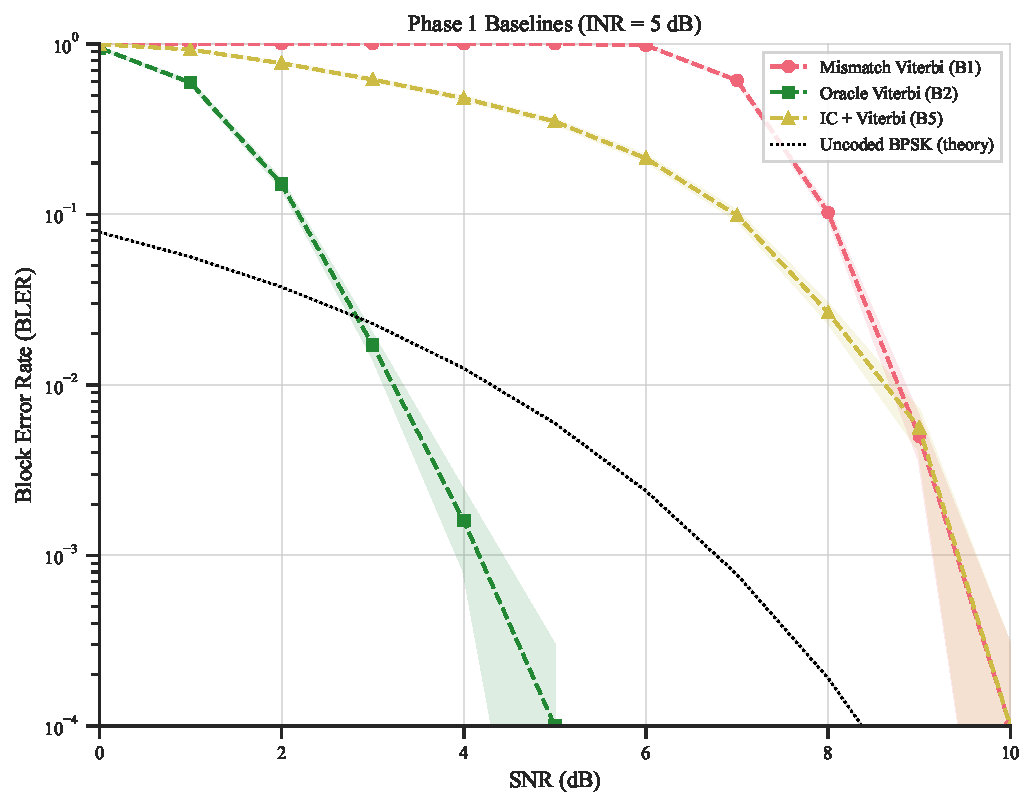
\includegraphics[width=\linewidth]{../results/phase1/figures/phase1_bler_vs_snr.pdf}
  \caption{BLER vs SNR at INR\,$=5$\,dB for the three classical baselines
  (B1, B2, B5).  B1 saturates; B2 is the oracle ceiling; B5 partially
  closes the gap before its estimator floor takes over near
  SNR\,$\approx 6$\,dB.}
  \label{fig:phase1_snr}
\end{figure}

\begin{figure}[t]
  \centering
  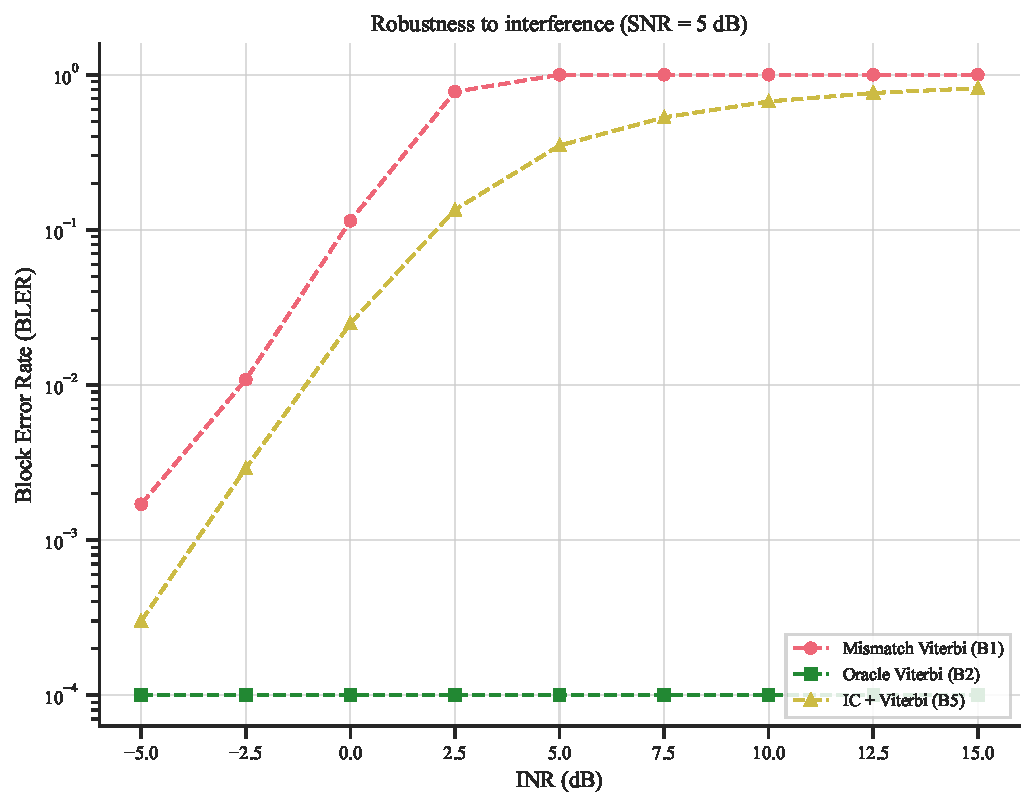
\includegraphics[width=\linewidth]{../results/phase1/figures/phase1_bler_vs_inr.pdf}
  \caption{BLER vs INR at SNR\,$=5$\,dB.  B2 is INR-invariant by
  construction; B1 saturates at BLER\,$=1$ for INR\,$\geq 5$\,dB; B5
  degrades as the estimator's residual error grows with interferer
  amplitude.}
  \label{fig:phase1_inr}
\end{figure}

\subsection{Neural Branch-Metric Decoder (N2)}
\label{sec:eval_n2}

Fig.~\ref{fig:n2_snr} compares both N2 training-target seeds against the
classical baselines on the SNR sweep.  Seed~32 reaches BLER\,$=2.5{\times}
10^{-3}$ at SNR\,$=5$\,dB---a gain exceeding five SNR-dB over B1 and
within $\approx 1.2$\,dB of B2 by log-linear interpolation
(B2 reaches the matched BLER at SNR\,$\approx 3.81$\,dB).  Seed~42, which
must absorb the $1/\sigma^2$ scaling into the network's output, sits
roughly $4$\,dB worse than seed~32 across the sweep and substantially
better than B1, demonstrating that training-target conditioning matters
even when the architecture and data are identical.

\begin{figure}[t]
  \centering
  \begin{subfigure}[b]{0.49\linewidth}
    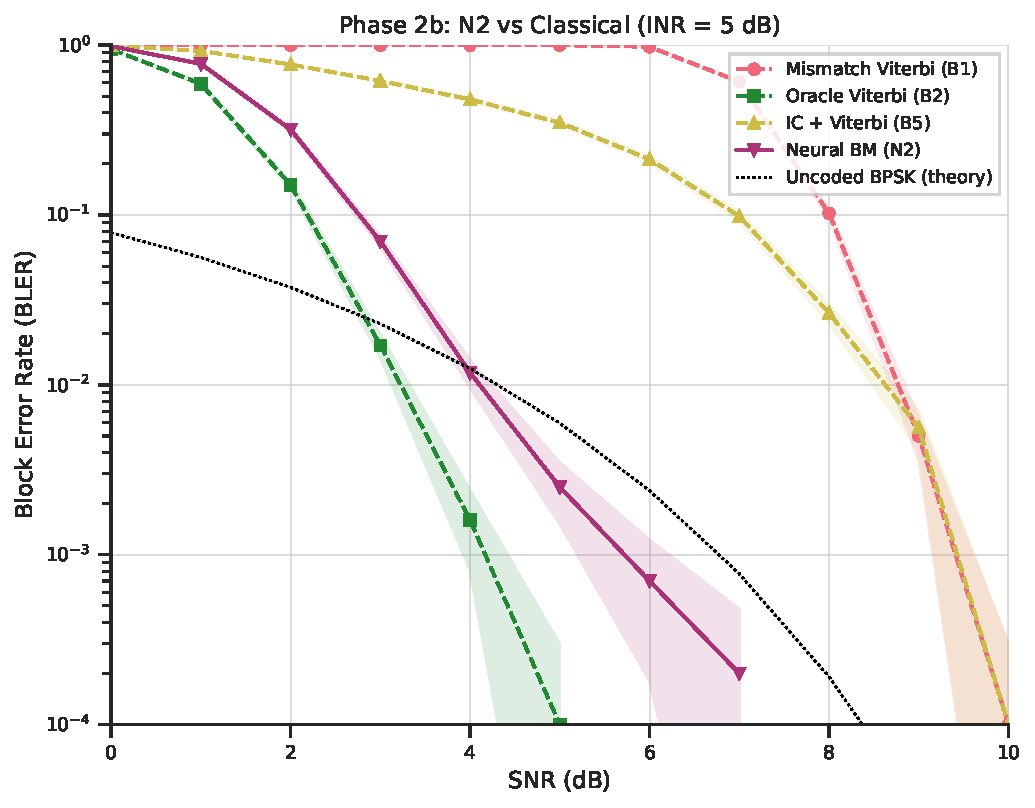
\includegraphics[width=\linewidth]{../results/phase2b/figures/phase2b_bler_vs_snr_seed32.pdf}
    \caption{Seed~32 (external $\sigma^2$ normalisation)}
    \label{fig:n2_snr_seed32}
  \end{subfigure}
  \hfill
  \begin{subfigure}[b]{0.49\linewidth}
    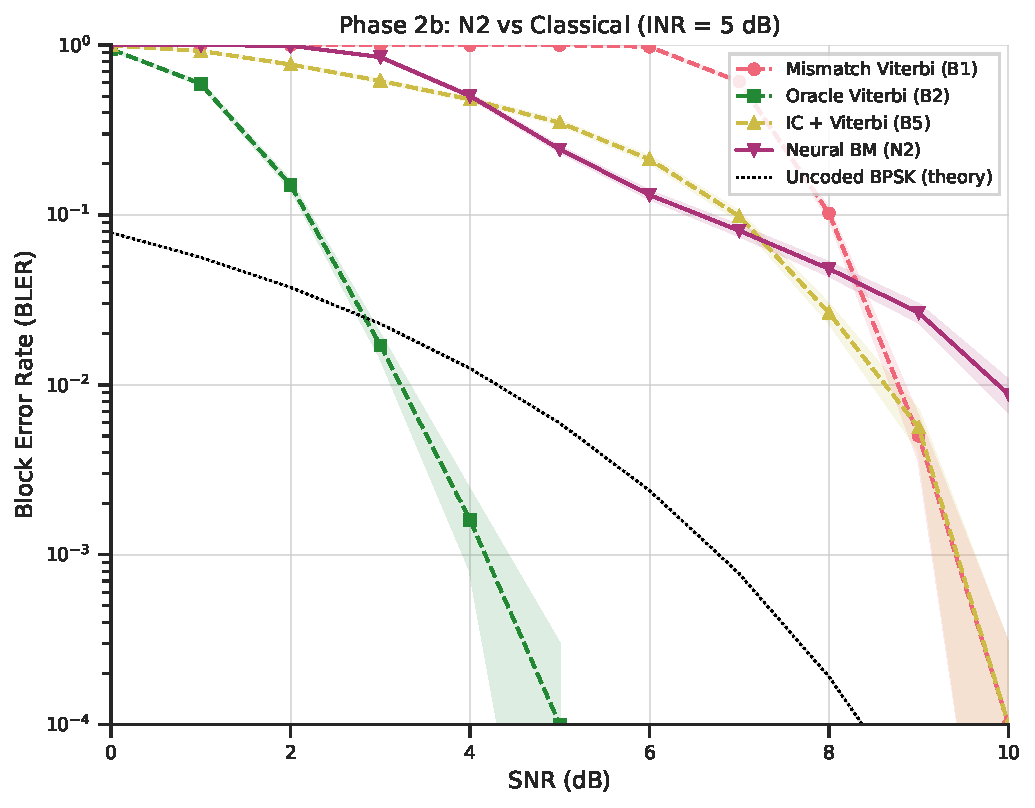
\includegraphics[width=\linewidth]{../results/phase2b/figures/phase2b_bler_vs_snr_seed42.pdf}
    \caption{Seed~42 (normalised targets)}
    \label{fig:n2_snr_seed42}
  \end{subfigure}
  \caption{N2 BLER vs SNR at INR\,$=5$\,dB for the two training-target
  variants, with B1/B2/B5 baselines.  Seed~32 closes most of the
  B1--B2 gap; seed~42's worse target conditioning leaves a several-dB
  residual.}
  \label{fig:n2_snr}
\end{figure}

Fig.~\ref{fig:n2_inr} plots the INR sweep at fixed SNR\,$=5$\,dB.
Seed~32 degrades \emph{gracefully}, holding BLER\,$<10^{-2}$ up to
INR\,$=10$\,dB and matching B1 exactly at INR\,$=-5$\,dB---a useful
sanity check that the learned metric reduces to the standard Euclidean
distance when interference vanishes.  B1 saturates at BLER\,$=1$ for
INR\,$\geq 5$\,dB; B5 deteriorates monotonically with INR.  Seed~42
saturates above INR\,$\approx 10$\,dB.

\begin{figure}[t]
  \centering
  \begin{subfigure}[b]{0.49\linewidth}
    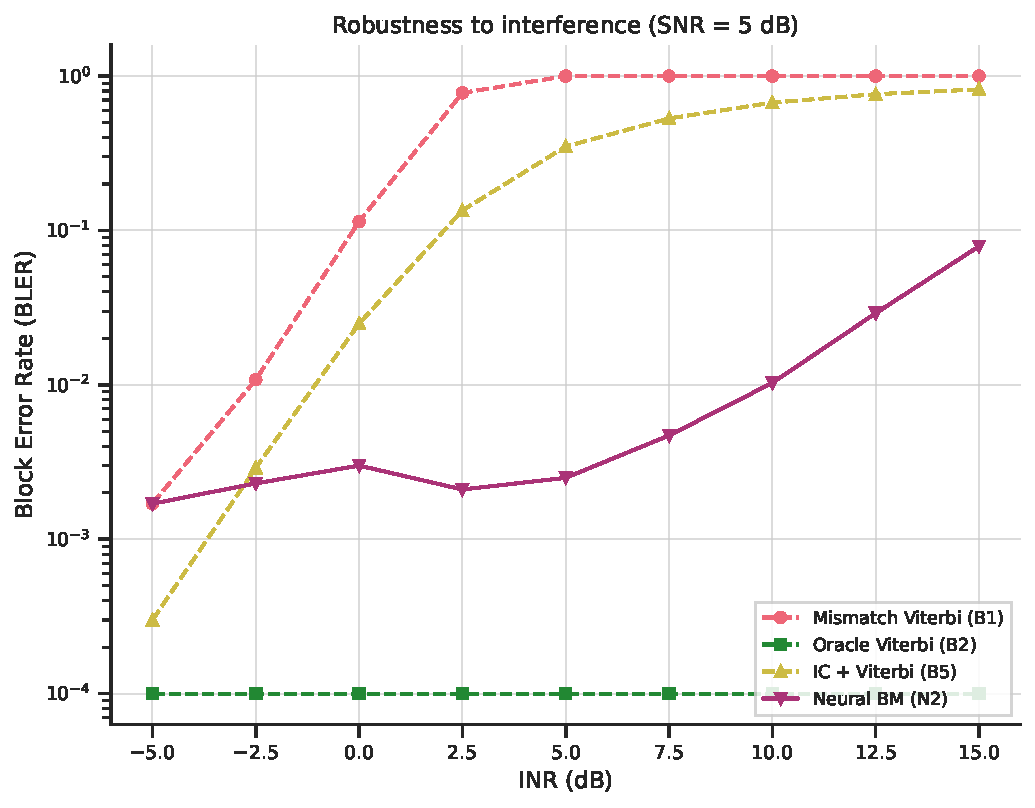
\includegraphics[width=\linewidth]{../results/phase2b/figures/phase2b_bler_vs_inr_seed32.pdf}
    \caption{Seed~32}
    \label{fig:n2_inr_seed32}
  \end{subfigure}
  \hfill
  \begin{subfigure}[b]{0.49\linewidth}
    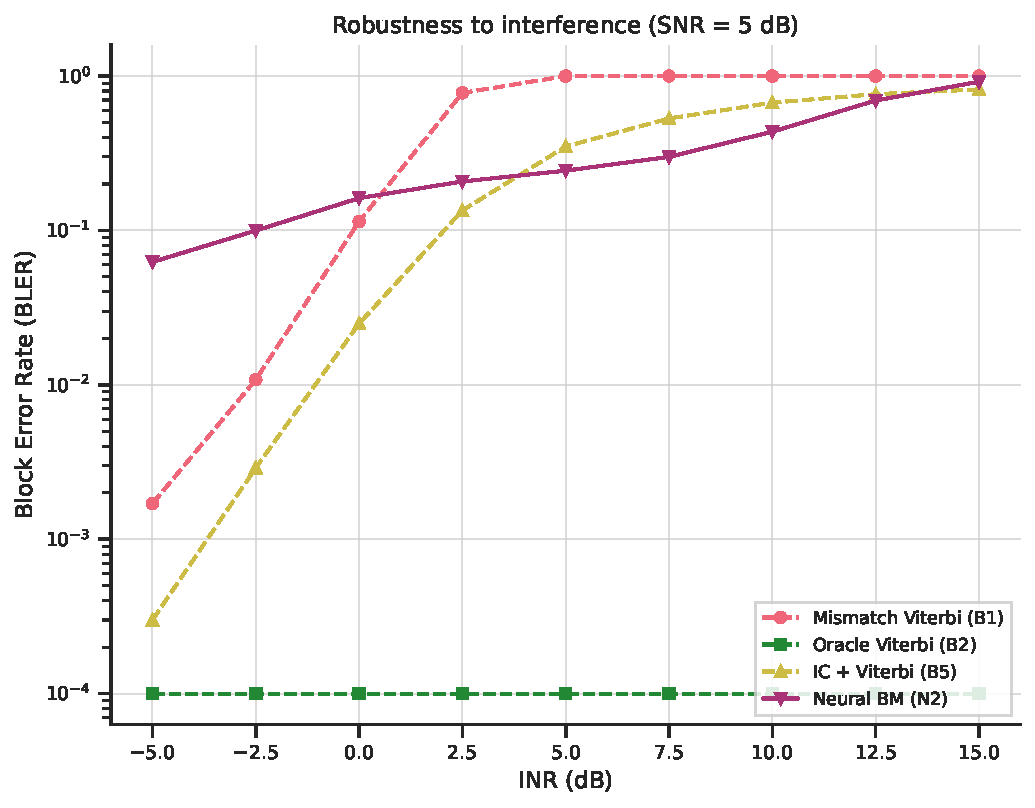
\includegraphics[width=\linewidth]{../results/phase2b/figures/phase2b_bler_vs_inr_seed42.pdf}
    \caption{Seed~42}
    \label{fig:n2_inr_seed42}
  \end{subfigure}
  \caption{N2 BLER vs INR at SNR\,$=5$\,dB.  Seed~32 degrades
  gracefully; B1 saturates above INR\,$\approx 5$\,dB.}
  \label{fig:n2_inr}
\end{figure}

\paragraph*{Training convergence.}
Table~\ref{tab:trainsummary} and Fig.~\ref{fig:trainhist} document the
training-target ablation.  Seed~32 starts at MSE\,$=24.4$ and reaches
$1.27$; seed~42's normalised-target formulation starts at MSE\,$=122.4$
and only reaches $18.97$ in the same epoch budget, with proportionally
worse validation BLER.  This is consistent with the Approach-section
argument that externalising the $1/(2\sigma^2)$ scaling decouples the
neural task (interference estimation) from the analytic noise scaling.

\begin{figure}[t]
  \centering
  \begin{subfigure}[b]{\linewidth}
    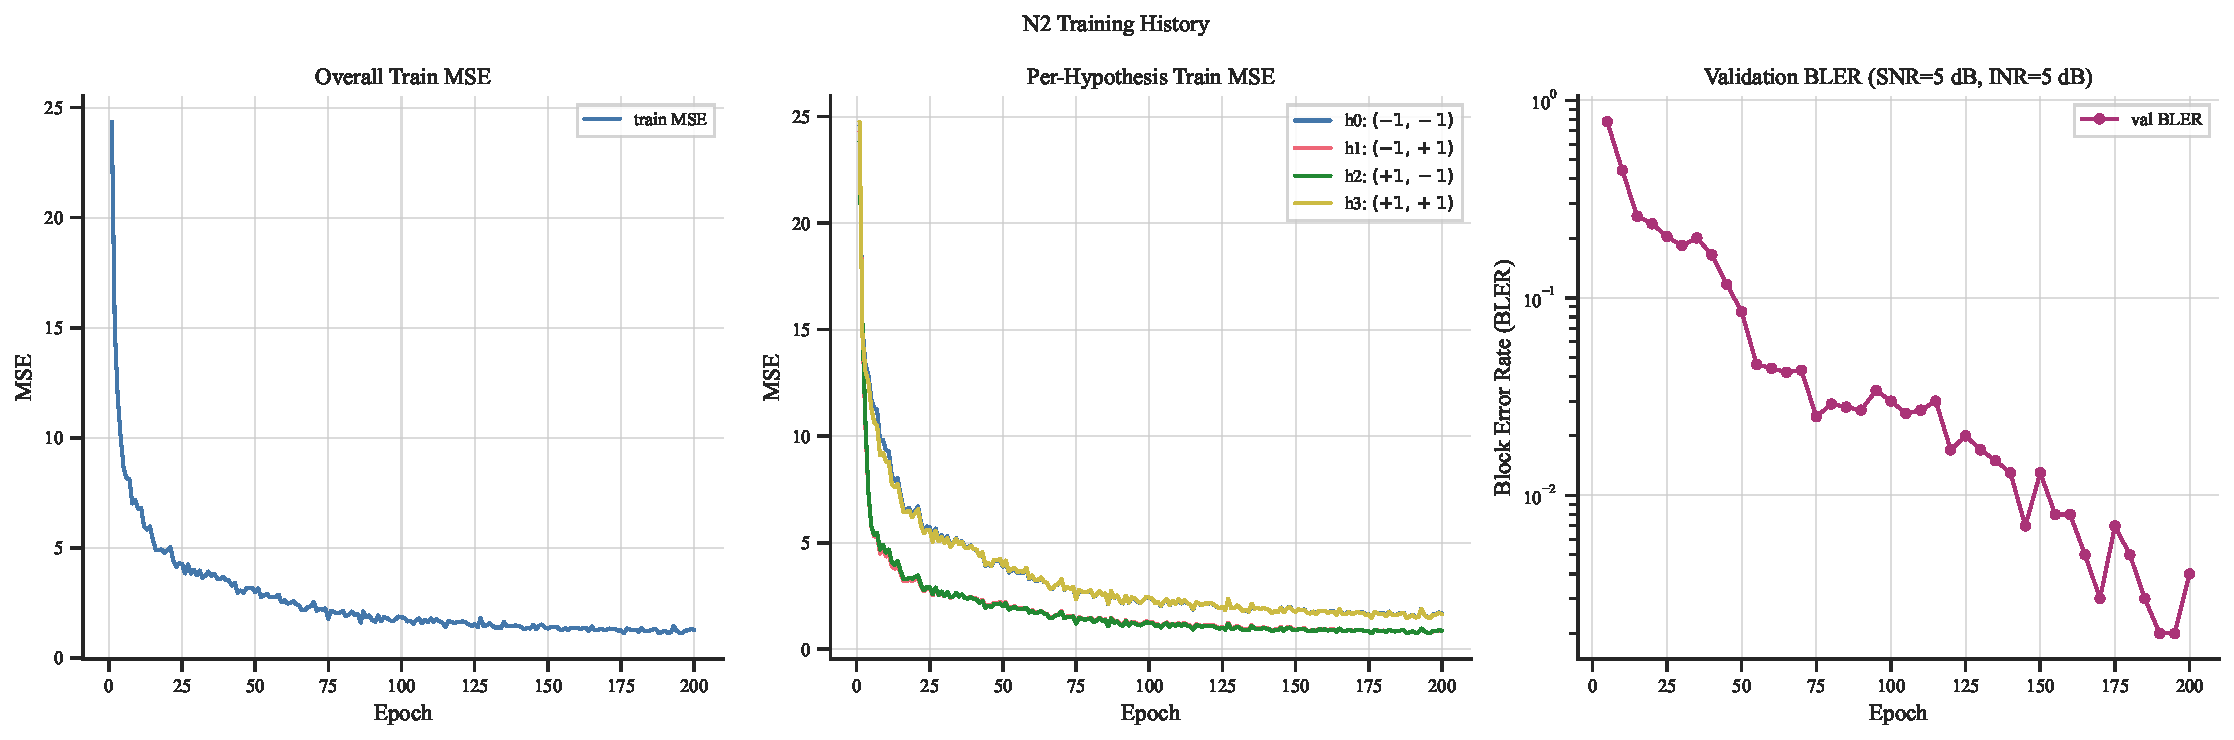
\includegraphics[width=\linewidth]{../results/phase2b/figures/training_history_seed32.pdf}
    \caption{Seed~32}
    \label{fig:hist_seed32}
  \end{subfigure}\\[1ex]
  \begin{subfigure}[b]{\linewidth}
    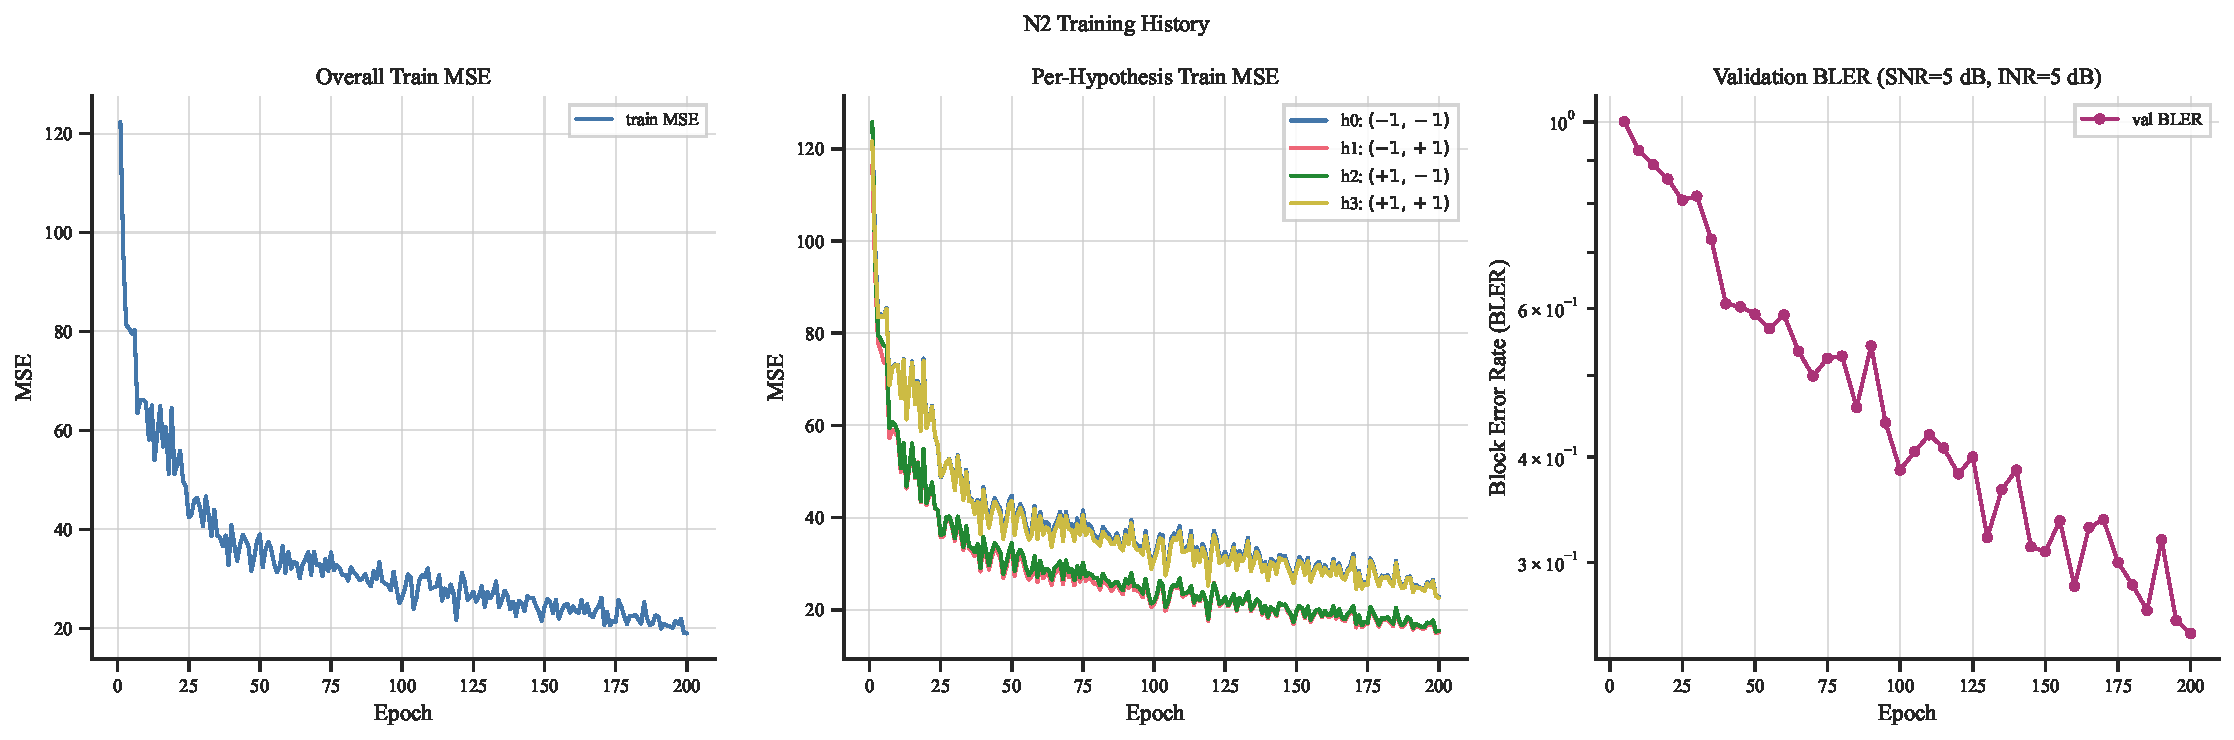
\includegraphics[width=\linewidth]{../results/phase2b/figures/training_history_seed42.pdf}
    \caption{Seed~42}
    \label{fig:hist_seed42}
  \end{subfigure}
  \caption{Per-epoch training MSE and validation BLER for both N2 seeds.
  Seed~32 converges substantially faster; summary in
  Table~\ref{tab:trainsummary}.}
  \label{fig:trainhist}
\end{figure}

\begin{table}[t]
  \centering
  \caption{N2 training convergence (best across $200$ epochs).}
  \label{tab:trainsummary}
  \footnotesize
  \setlength{\tabcolsep}{4pt}
  \begin{tabular}{lrrrr}
    \toprule
    Seed & Init.\ MSE & Final MSE & Best val.\ BLER & Best epoch \\
    \midrule
    32 & $24.4$  & $1.27$  & $0.002$ & $190$ \\
    42 & $122.4$ & $18.97$ & $0.247$ & $200$ \\
    \bottomrule
  \end{tabular}
\end{table}

\subsection{Evolutionary Trellis Search}
\label{sec:eval_ea}

\paragraph*{Phase~3a (oracle fitness).}
Seed~$0$ converges over $34$ generations: best-genome BLER drops
monotonically from $2.1{\times}10^{-2}$ (gen.~0) to $1.1{\times}10^{-2}$
(gen.~23), then plateaus until early stop at gen.~33.  Full evaluation
of the best genome at $100{,}000$ trials yields BLER\,$=8{\times}10^{-5}$
at SNR\,$=5$\,dB---within Monte-Carlo noise of B2's
$10^{-4}$---confirming that the EA reproduces the matched-decoder
benchmark and that the constraint checks are not over-restrictive.  I
omit a separate Phase~3a figure because its BLER vs SNR/INR curve is
indistinguishable from B2's at the trial counts used.

\paragraph*{Phase~3b (frozen-N2 fitness).}
The fitness curve in Fig.~\ref{fig:phase3b}\,(left) shows immediate
convergence at generation~1, after which no mutation improved the best
genome over $11$ generations until plateau.  I compared the best genome
to NASA~K=7 element-wise on both the next-state and output-pair tables
and verified an exact SHA-256 match: the EA \emph{recovers} NASA~K=7 as
the optimal trellis under N2 decoding.  Fig.~\ref{fig:phase3b}\,(right)
confirms that the resulting BLER vs SNR curve coincides with N2 on
NASA~K=7 within Monte-Carlo noise.  This is a striking result: under
two independently-defined fitness functions (one analytical, one
learned), the EA returns the same trellis the engineering community has
used for half a century.  Section~\ref{sec:discussion} interprets this
finding.

\begin{figure}[t]
  \centering
  \begin{subfigure}[b]{0.49\linewidth}
    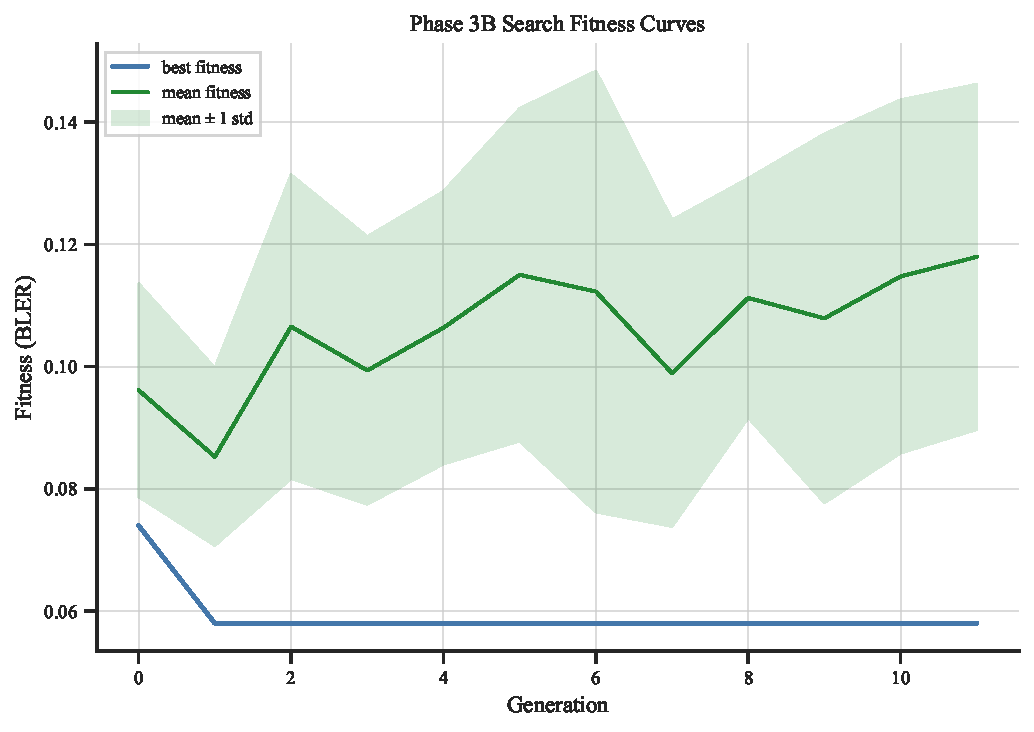
\includegraphics[width=\linewidth]{../results/phase3b/figures/fitness_curves_seed0.pdf}
    \caption{Phase~3b EA fitness}
    \label{fig:phase3b_fitness}
  \end{subfigure}
  \hfill
  \begin{subfigure}[b]{0.49\linewidth}
    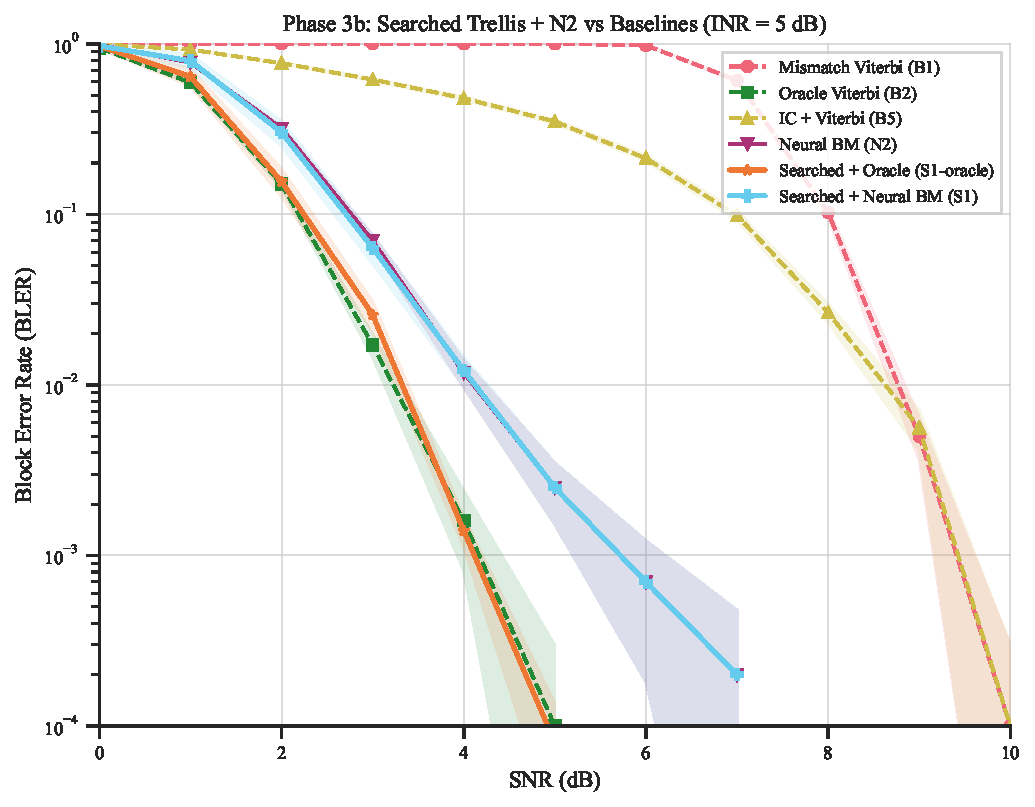
\includegraphics[width=\linewidth]{../results/phase3b/figures/phase3b_bler_vs_snr.pdf}
    \caption{S1 (search + N2) vs N2 (NASA + N2)}
    \label{fig:phase3b_snr}
  \end{subfigure}
  \caption{Phase~3b convergence and BLER.  The EA converges in a single
  generation to NASA~K=7 (verified by element-wise and SHA-256 match);
  the resulting BLER curve is indistinguishable from N2 on NASA~K=7
  within MC noise.}
  \label{fig:phase3b}
\end{figure}

\subsection{Compute Cost and Operating-Point Summary}

Table~\ref{tab:compute} merges per-method compute into a single budget
view.  All admissible methods consume $\leq 43.5\%$ of the $2.1$~MFLOP
budget; only the rejected end-to-end N1 violates it.  Wall-clock
latencies reflect unoptimised Python/PyTorch CPU inference and should
not be compared across implementations; the FLOP column is the
budget-relevant quantity.  Table~\ref{tab:summary} summarises BLER and
compute at the headline operating point.

\begin{table}[t]
  \centering
  \caption{Per-block compute cost (single block, $\%$ of $2.1$\,MFLOP
  budget).  Latencies are unoptimised CPU PyTorch and are
  cross-method-incomparable.}
  \label{tab:compute}
  \small
  \begin{tabular}{lrrr}
    \toprule
    Method & FLOPs & Lat.\ (ms) & \% budget \\
    \midrule
    B1 mismatched Viterbi & $65{,}536$  & $0.30$ & $3.1\%$ \\
    B2 oracle Viterbi     & $65{,}536$  & $0.35$ & $3.1\%$ \\
    B5 IC + Viterbi       & $94{,}720$  & $1.24$ & $4.5\%$ \\
    N1 end-to-end (rejected) & $6{,}640{,}000$ & --- & $317\%$ \\
    N2 seed~32            & $913{,}664$ & $1981.9$ & $43.5\%$ \\
    N2 seed~42            & $913{,}664$ & $1614.2$ & $43.5\%$ \\
    S1-oracle (Phase~3a)  & $65{,}536$  & --- & $3.1\%$ \\
    S1 (Phase~3b)         & $913{,}664$ & --- & $43.5\%$ \\
    \bottomrule
  \end{tabular}
\end{table}

\begin{table}[t]
  \centering
  \caption{Summary at SNR\,$=$\,INR\,$=5$\,dB.  Methods sorted by BLER.}
  \label{tab:summary}
  \small
  \begin{tabular}{lrrr}
    \toprule
    Method & BLER & FLOPs & \% budget \\
    \midrule
    B2 oracle Viterbi   & $1.0\times10^{-4}$ & $65{,}536$  & $3.1\%$ \\
    S1-oracle (Phase~3a) & $8\times10^{-5}$  & $65{,}536$  & $3.1\%$ \\
    N2 seed~32          & $2.5\times10^{-3}$ & $913{,}664$ & $43.5\%$ \\
    S1 (Phase~3b)       & $2.5\times10^{-3}$ & $913{,}664$ & $43.5\%$ \\
    N2 seed~42          & $2.4\times10^{-1}$ & $913{,}664$ & $43.5\%$ \\
    B5 IC + Viterbi     & $3.5\times10^{-1}$ & $94{,}720$  & $4.5\%$ \\
    B1 mismatched       & $1.0$              & $65{,}536$  & $3.1\%$ \\
    \bottomrule
  \end{tabular}
\end{table}

% ============================================================
\section{Discussion and Limitations}
\label{sec:discussion}

\subsection{Why the EA Returns NASA K=7}
N2 is trained to regress the oracle log-likelihood
$-\norm{\mathbf{y}[k]-\mathbf{h}_j-\mathbf{i}[k]}^2$ at each trellis step,
which is exactly the quantity that makes oracle Viterbi optimal.  A
decoder whose branch metrics approximate oracle log-likelihoods will
benefit most from a trellis that is optimal under oracle decoding---and,
for $64$-state rate-$1/2$ codes with $\dfree\geq 8$, that trellis is
NASA~K=7 within the search budget I explored.  The two-fitness
convergence (oracle in Phase~3a, learned in Phase~3b) is therefore
mutually consistent rather than coincidental: a learned metric that
faithfully tracks the analytical optimum inherits its trellis preference.
I frame this as evidence that NASA~K=7 \emph{is near-optimal in this
setting}, not that it is globally optimal: the result is conditioned on a
frozen N2 decoder, the constraint set listed in Section~\ref{sec:ea}, and
single-seed EA runs.

\subsection{Limitations}
\label{sec:limitations}
\begin{enumerate}
  \item \emph{Synthetic channel.}  The interferer is generated from a
    parametric sinusoidal model; I did not validate against measured
    industrial-band traces.
  \item \emph{Single trellis depth.}  Only $K_c = 7$ is studied;
    behaviour at longer constraint lengths may differ.
  \item \emph{Single interference family.}  Generalisation to chirp,
    pulsed, or multitone interferers has not been characterised.
  \item \emph{Frozen-decoder search.}  Phase~3 freezes N2 during the EA;
    a jointly-retrained decoder might prefer a non-NASA trellis that
    exploits interference patterns the standard linear code cannot
    express.
  \item \emph{Single-seed EA.}  Phases~3a/3b each report one EA seed;
    coefficient-of-variation across seeds remains to be established.
  \item \emph{Out-of-distribution interference.}  N2 is trained over
    $P\in[8,32]$; performance on shorter or longer periods has not been
    measured.
  \item \emph{Wall-clock latency.}  N2 latency under unoptimised
    PyTorch CPU inference is two orders of magnitude above what the
    FLOP budget would permit on optimised hardware; the FLOP column is
    the budget-relevant figure.
\end{enumerate}

\subsection{Future Work}
Two directions follow directly.  \emph{Joint co-design}: re-train N2
against the searched trellis rather than freezing the Phase~2b
checkpoint may yield a non-NASA optimum.  \emph{Wider channel
distributions}: training and evaluating on chirp, multi-tone, and
measured industrial-band interferers will test the robustness of the
local-channel-estimation hypothesis.

% ============================================================
\section{Conclusion}
\label{sec:conclusion}

A small ($\approx 1.86$\,k-parameter) BiGRU branch-metric estimator
plugged into a standard Viterbi decoder closes most of the gap to the
oracle bound under periodic sinusoidal interference at $43.5\%$ of a
strict $2.1$\,MFLOP/block compute budget.  The architectural lesson is
the decomposition of \emph{local channel estimation} (neural) from
\emph{global trellis search} (classical algorithm); a budget-violating
end-to-end alternative fails to learn.  Evolutionary search over valid
$64$-state rate-$1/2$ trellises returns NASA~K=7 under both oracle and
frozen-N2 fitness, providing empirical evidence that the classical
benchmark is near-optimal for this decoder class in this setting.

% ============================================================
\bibliographystyle{IEEEtran}
\begin{thebibliography}{9}

\bibitem{viterbi1967}
A.~J. Viterbi,
``Error bounds for convolutional codes and an asymptotically optimum decoding
algorithm,''
\emph{IEEE Trans. Inf. Theory}, vol.~13, no.~2, pp.~260--269, Apr.~1967.

\bibitem{proakis2008}
J.~G. Proakis and M.~Salehi,
\emph{Digital Communications}, 5th~ed.
McGraw-Hill, 2008.

\bibitem{nasastandard}
J.~A. Heller and I.~M. Jacobs,
``Viterbi decoding for satellite and space communication,''
\emph{IEEE Trans. Commun. Technol.}, vol.~19, no.~5, pp.~835--848, Oct.~1971.

\bibitem{hagenauer1989}
J.~Hagenauer and P.~Hoeher,
``A Viterbi algorithm with soft-decision outputs and its applications,''
in \emph{Proc. IEEE GLOBECOM}, Dallas, TX, Nov.~1989, pp.~1680--1686.
% TODO author/student: confirm full venue formatting.

\bibitem{shlezinger2020}
N.~Shlezinger, N.~Farsad, Y.~C. Eldar, and A.~J. Goldsmith,
``ViterbiNet: A deep learning based Viterbi algorithm for symbol detection,''
\emph{IEEE Trans. Wireless Commun.}, vol.~19, no.~5, pp.~3319--3331, May~2020.

\bibitem{nachmani2018}
E.~Nachmani, E.~Marciano, L.~Lugosch, W.~J. Gross, D.~Burshtein, and Y.~Be'ery,
``Deep learning methods for improved decoding of linear codes,''
\emph{IEEE J. Sel. Topics Signal Process.}, vol.~12, no.~1, pp.~119--131, Feb.~2018.

\bibitem{gruber2017}
T.~Gruber, S.~Cammerer, J.~Hoydis, and S.~ten Brink,
``On deep learning-based channel decoding,''
in \emph{Proc. 51st Annu. Conf. Inf. Sci. Syst. (CISS)}, Baltimore, MD,
Mar.~2017.

\bibitem{kim2018}
H.~Kim, Y.~Jiang, R.~Rana, S.~Kannan, S.~Oh, and P.~Viswanath,
``Communication algorithms via deep learning,''
in \emph{Proc. Int. Conf. Learning Representations (ICLR)}, Vancouver,
Apr.~2018.

\bibitem{kargi2024}
T.~Kargi and T.~M. Duman,
``A deep learning based decoder for concatenated coding over deletion channels,''
in \emph{Proc. IEEE Int. Conf. Commun. (ICC)}, Denver, CO, Jun.~2024.

\bibitem{yang2022}
Z.~Yang and Y.~Jiang,
``Online learning of trellis diagram using neural network,''
arXiv:2202.10635, Feb.~2022.

\end{thebibliography}

% TODO before submission:
%   1. Add a real industrial-IoT / VFD-emissions citation to ground the
%      sinusoidal-interference channel model in Section II / Implementation
%      "simulation realism" paragraph.  Suggested search: IEEE Trans. EMC
%      papers on conducted/radiated emissions from variable-frequency drives.
%   2. Make https://github.com/akmanjun-usc/Research public (or change the
%      URL footnote to a public mirror).
%   3. Verify hagenauer1989 and nachmani2018 bibliographic details
%      against the canonical IEEE citation style; both are real papers but
%      please double-check pages and venue formatting.

\end{document}
